\documentclass[11pt,a4paper,twoside]{article}
\usepackage{tascar}
\pagenumbering{arabic}
\pagestyle{empty}
\showtutorialtrue
\begin{document}
\setcounter{tutorial}{3}
\begin{tutorial}{Room acoustic modeling, diffuse sources and reverberation}{VR-Lab, seminar room}

In this session you will learn how to create a room acoustical
environment in \tascar{}.
%
You will define room dimensions, surfaces, obstacles and reverberation
parameters and experience their effect on direct and diffuse
sounds.
%
The presented tools are useful for applications like VR scenarios for
hearing aid evaluation or investigations of the influence of room
acoustical parameters on hearing.

\begin{learnitems}
\item How to simulate room acoustics in \tascar{}
\item How to render impulse responses
\item Concept of diffuse reverberation in \tascar{}
\end{learnitems}

\begin{appitems}
\item Measure influence of early reflections on hearing aid performance
\item Increase complexity of virtual acoustic environments
\end{appitems}

\medskip

\centerline{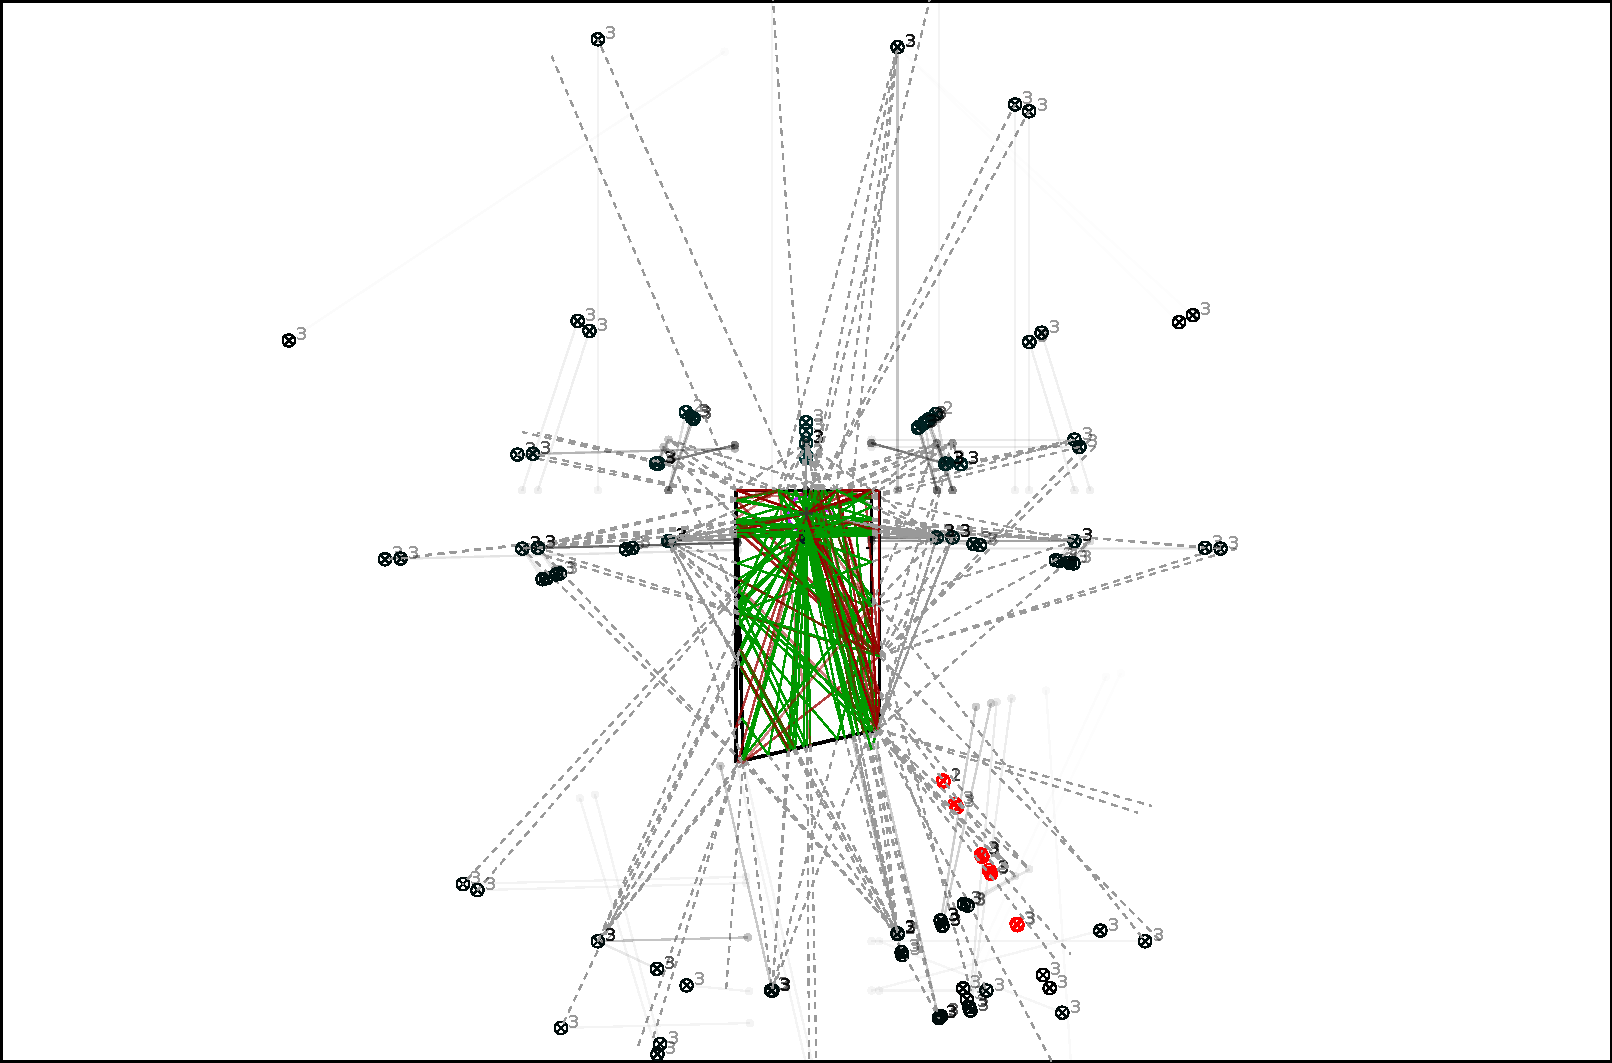
\includegraphics[width=0.9\columnwidth]{t4_acmodel}}

\end{tutorial}

\ifshowtutorial

\newpage

\subsection*{Different Types of Sound Sources and Signal Paths in TASCAR}
\begin{itemize}
\item Make a copy of file \verb!task4_basic.tsc! in text editor. Then load
  your scene in TASCAR.
\item Identify the three scenes in the session. Have a look the
  receivers. How many receivers are there? What is the purpose of each
  receiver?
\item Look at the jack signal graph (e.g., with patchage, type Ctrl-R
  to reload, and Ctrl-G to reorder).
\item As you remember from the introduction, diffuse sources are
  rendered in first order Ambisonics and require four-channel audio
  signals. Identify diffuse signals in both scenes.
\item zita-rev1 is a feedback delay network (FDN) reverberation tool
  (to be replaced by RaZRTM in the future).
\item Can you change late reverberation from FDN to convolution
  reverb? You can use the impulse response
  \verb!diff_nuclear_b_format.wav!  in the tutorial4 folder or look
  for other impulse responses in \verb!~/tascar_scenes/diffusereverb!
  or on \url{http://www.openairlib.net/}.
\item Listen carefully to the diffuse background and diffuse
  reverberation. Are they diffuse?  What happens if you move your
  head?
\end{itemize}

\subsection*{Surfaces and Their Properties}
  
\begin{itemize}
\item Have a look at the elements face, facegroup and obstacle. How
  was the movement of ``thewall'' defined?
\item Create a movement of a sound source or a receiver using one of
  the tools described in the manual sections 6.6 – 6.8.
\item Open your copy of a file \verb!task4_basic.tsc! in text editor.
\item Open script \verb!task4_example1.m! in MATLAB or GNU Octave (to
  open MATLAB, please open a terminal and type \verb!matlab &!).
\item Modify the reflectivity and damping properties of surfaces in
  your copy of \verb!task4_basic.tsc!.
\item Using this example, see how easy you can render impulse
  responses and image source model. If external modules
  (e.g. zita-rev1, jconvolver) shall be included, you can use
  \verb!tascar_jackio!.
\end{itemize}


\fi
\end{document}
